\newpage
%TODO : Contexte de votre sujet
%TODO : L'organisation
%TODO : l'objectif de l'étude
%TODO : les enjeux pour l'entreprise

\section{Contexte du stage} % (2 pages) Entreprise, service, mission
Le stage se déroule au sein de l'entreprise SUPRALOG, du groupe IDLOG.

\subsection{Le groupe IDLOG}
\gls{IDLOG} est un groupe familial créé en 2002 afin de regrouper les sociétés \gls{SUPRALOG} créée en 1997 et \gls{IDEA} créée en 1987.\\
Il réuni les activités d'intégration de technologies, d’édition de progiciels et d'assistance aux utilisateurs.
%Le groupe exerce une diversité de métiers complémentaires : 
%\begin{itemize}
%\item Edition et diffusion de gammes de progiciels.
%\item Assistance utilisateurs et centre d'appels.
%\item Ecommerce B2B et B2C.
%\item Intégration de technologies et élaboration de solutions sur mesure.
%\item Consulting IT.
%\item Formations spécifiques (centre de formation agréé).
%\end{itemize}

\subsection{Entreprise}
Supralog est un éditeur de logiciels avec une activité de conseil en systèmes d'information créée en 1997.
L'entreprise compte 45 collaborateurs et est implantée sur la technopole de Sophia Antipolis.

\begin{figure}[H]
  \centering
  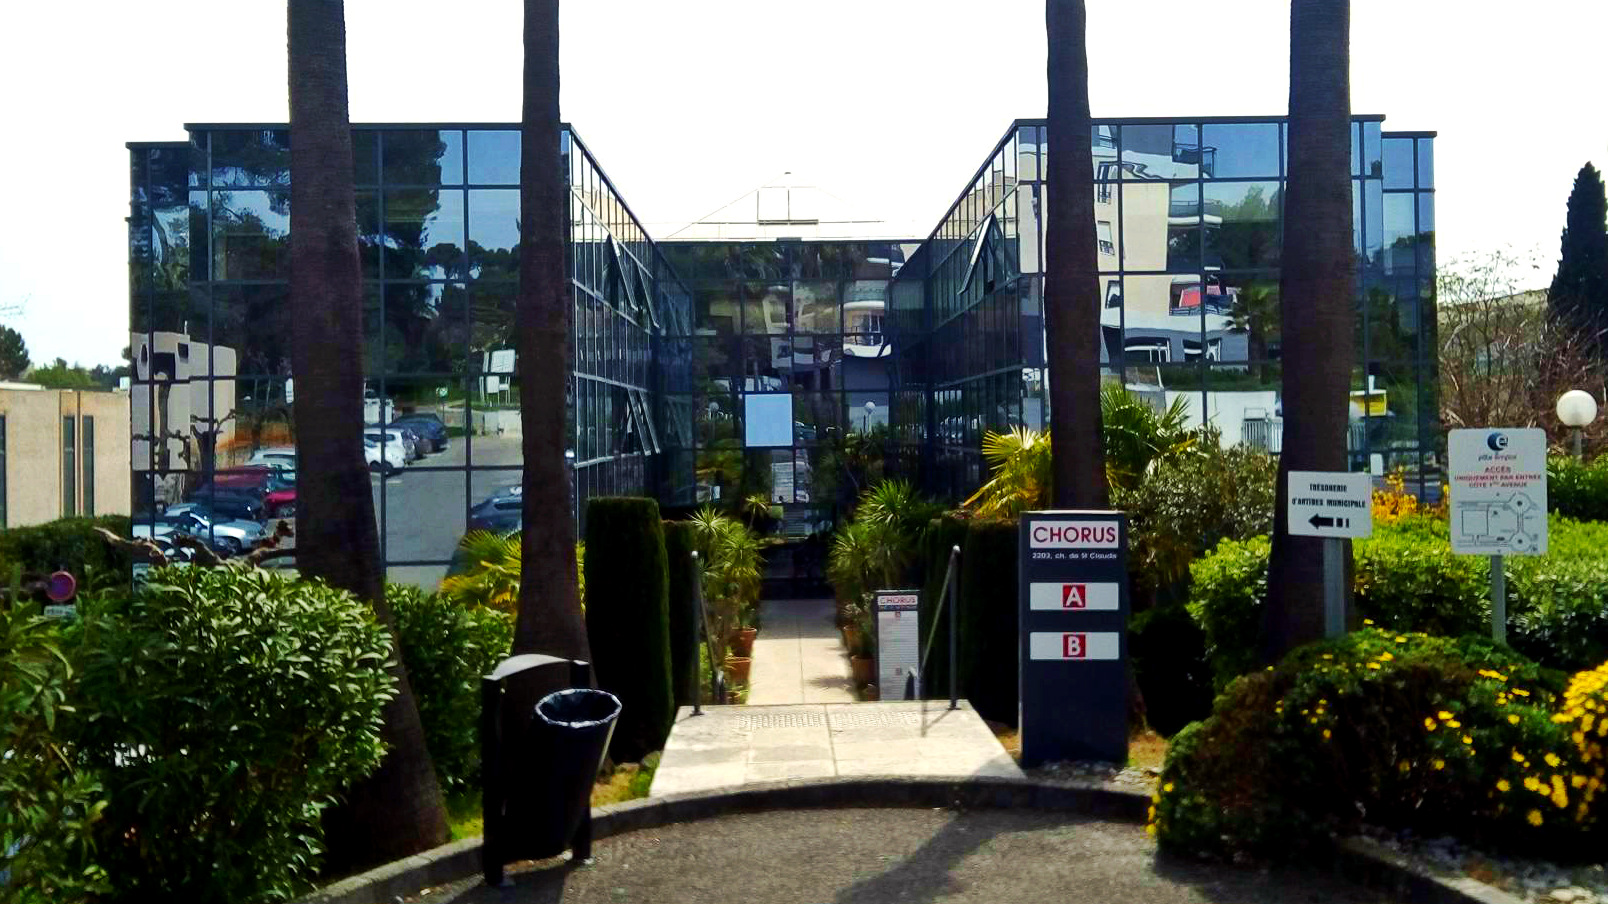
\includegraphics[width=9cm]{./img/supralog_building_3}
  \caption{\label{fig:mb_va_ast} Supralog}
\end{figure}


\paragraph{Les trois activités de l'entreprise\\}
Supralog est organisé en trois practices : Progiciel / Technologie / Conseil.\\
L'activité historique est l'édition de progiciels. Supralog développe deux gammes de solutions:
\begin{sitemize}
\item \textit{Topaze} qui permet la gestion des cabinets médicaux.
\item \textit{Intr@ssoc} qui est destiné à la gestion des grandes associations et fédérations.
\end{sitemize}

La deuxième activité de l'entreprise est le conseil, notamment pour \textit{Air France} et \textit{Amadeus}.\\
Enfin, il y a l'activité technologie qui porte sur la conception et le développement de systèmes d'information, au forfait, chez Supralog. 

\paragraph{Quelques chiffres\\}
Les progiciels développés par SUPRALOG sont utilisés par plus de 40 000 personnes en France.\\
Les activités de technologie et de conseil regroupent plus de 15 clients.\\
L'entreprise a réalisé un chiffre d'affaires de plus de 7 millions d'euros en 2014 et présente une croissance de 114\% sur les 3 dernières années.

\subsection{Environnement de travail}
Mon stage se déroule au siège de l'entreprise au sein de l'équipe de développement du projet \textit{Topaze Web}.
L'équipe est constituée de 5 personnes : le chef de projet et directeur technique Nicolas Thibault, les ingénieurs développeurs Abdessalam Eljai et Anthony Biga, l'apprenti Tom Veniat et moi-même.

\subsection{Le projet Topaze Web et la gamme Topaze}
Topaze est une gamme de progiciels de gestion de cabinets pour professionnels des milieux
médicaux et paramédicaux. Cette gamme a été créée par Supralog en 1997 et est historiquement le
premier progiciel de santé à obtenir l'agrément SESAM Vitale, agrément permettant l’édition de
feuilles de soins électroniques.\\

Depuis 1997, Topaze a connu de nombreuses évolutions et a été publié et agréé en plusieurs versions ayant des architectures différentes. Lors de sa création Topaze était une application de bureau, puis il a évolué progressivement pour s'ouvrir à internet.
 
En 2015, le projet Topaze Web a été initié avec comme objectif de donner naissance à une application web multi-tiers offrant les mêmes fonctionnalités que la version "Maestro" de Topaze.

%Ce projet, lancé en 2015, a pour objectif de permettre aux utilisateurs d’accéder au logiciel directement depuis leur
%navigateur web. Cette solution cloud possède différents avantages par rapport aux solutions classiques.
%Il n’est tout d’abord plus nécessaire d’installer un client lourd sur chaque poste utilisé par le
%professionnel de santé. Les risques de pertes de données ont été réduits ; cette architecture est déjà
%présente sur certaines versions de Topaze. En effet, les données étant stockées sur une machine
%distante, le dysfonctionnement de la machine d’un utilisateur n’impactera d’aucune manière ses
%données qui resteront accessibles depuis n’importe quel autre ordinateur se connectant à son compte.
%Au début de l’apprentissage, le projet Topaze Web avait déjà commencé depuis plusieurs
%mois. Il s’agit d’un projet utilisant majoritairement la spécification Java Enterprise Edition (J2EE) en
%combinaison avec les Frameworks Hibernate, Spring et JavaServer Faces (JSF).
%Les spécifications de l’application à réaliser sont basées sur l'existant : Topaze Web devra
%fournir des fonctionnalités similaires à celles de Topaze Maestro (version de Topaze initialement
%lancée en 2011). Tout en modernisant le design, l’interface utilisateur devra être suffisamment proche
%de celle de Topaze Maestro pour que les utilisateurs qui migreront prennent rapidement en main la
%nouvelle version. C’est dans ce cadre que cet apprentissage a débuté au sein de l’équipe de
%développement en charge de la réalisation de Topaze Web, composée d’un chef de projet et de deux
%autres développeurs.
%Le fonctionnement au sein de cette équipe suit les méthodologies agiles. Les fonctionnalités à
%développer en priorité sont choisies par le client, représenté par un membre de l’entreprise
%commercialisant Topaze. Le client suit étape par étape l’avancement du projet ce qui permet à l’équipe
%d’obtenir des retours réguliers.
%Ce rapport commencera par présenter plus précisément le projet, son contexte et ses objectifs
%avant d’exposer les problèmes posés au cours de cette première période d’apprentissage. Les attentes
%et le contexte dans lequel chaque mission s’inscrit y sont détaillés. La seconde partie exposera le
%travail réalisé, en expliquant plus précisément les méthodes employées pour remplir les missions qui
%ont été confiées. La démarche suivie ainsi que les résultats y sont décrits. La conclusion contient le
%bilan de cette première partie de l’année, ainsi que les compétences développées au cours de ces 2
%mois.

\subsection{Mission}
Mon rôle au sein de \textit{Topaze Web} est de me familiariser avec l'architecture du projet et ses technologies (\gls{Java EE}, \gls{Hibernate}, \gls{Spring} et \gls{JSF}) et de participer à la conception et au développement de l'application.\\

Les spécifications de l’application à réaliser sont basées sur l'existant : Topaze Web devra fournir des fonctionnalités similaires à celles de Topaze Maestro. Le design de l'application doit être modernisé, mais son ergonomie doit rester proche de l'existant pour ne pas déstabiliser l'utilisateur final. Enfin, un soin particulier doit être accordé à l'architecture, la conception et l'utilisation de patrons de conception lors du développement de l'application, afin de garantir la pérennité et la maintenabilité du logiciel au cours du temps. 

%Il s’agit d’un projet utilisant majoritairement la spécification Java Enterprise Edition (J2EE) en
%combinaison avec les Frameworks Hibernate, Spring et JavaServer Faces (JSF).
%Les spécifications de l’application à réaliser sont basées sur l'existant : Topaze Web devra
%fournir des fonctionnalités similaires à celles de Topaze Maestro (version de Topaze initialement
%lancée en 2011). Tout en modernisant le design, l’interface utilisateur devra être suffisamment proche
%de celle de Topaze Maestro pour que les utilisateurs qui migreront prennent rapidement en main la
%nouvelle version. C’est dans ce cadre que cet apprentissage a débuté au sein de l’équipe de
%développement en charge de la réalisation de Topaze Web, composée d’un chef de projet et de deux
%autres développeurs.

%TODO : Refactorer ou virer 
%\paragraph{Gestion de projet\\}
%La gestion du projet se fait en mode agile, selon une méthodologie proche du Scrum. 
%Les fonctionnalités à développer en premier son choisies par le client (la société IDEA d'IDLOG), puis les tâches sont chiffrées et réparties par le chef de projet. Le logiciel \textit{Jira} est utilisé pour l'assignation et le suivi des tâches. \\
%À la fin de chaque sprint, une réunion est organisé avec le client afin de montrer l'évolution du projet.


